\chapter*{Introduction}\addcontentsline{toc}{chapter}{Introduction}
Knowing the Earth's topography is crucial for modern geosciences. Depending on the level of details needed, different models can be used: the Earth ellipsoid, its geoid (gravity equipotential surface), contour lines on hiking maps \etc One of those models are , \acrfull{dsm}, which are a representation of a surface's elevation on a regular grid. This type of model appears as a natural solution in many \acrfull{gis}. Indeed, they can easily be handled and provide georeferenced information regarding the topography of an area. Figure \ref{fig:intro_dsm_example} presents an example of a DSM.

\acrshort{dsm} find usage in various contexts and for a wide range of applications. In \acrfull{eo} for instance, \acrshort{dsm} are used to monitor changes in vegetation \cite{sadeghi_canopy_2016}, melting rates of glaciers \cite{berthier_glacier_2014, rieg_pleiades_2018}, volcanos \cite{ganci_data_2022}, snow or water resources \cite{marti_mapping_2016, gascoin_theia_2019, yamazaki_merit_2019} \etc Similarly, \acrshort{dsm} are employed for catastrophe management, to predict the potential damage caused by earthquakes or floods \cite{jenkins_physics-based_2023} \etc \acrshort{dsm} are also crucial for ortho-rectifying images, \ie geometrically correcting the effects of distortions between the sensor and the terrain. This process creates a planimetric image with a consistent scale in all parts of the image. It allows images to be easily used in GIS or as background for maps. Finally, high resolution \acrshort{dsm} can help drone navigation in urban settings, for Defense applications, or more broadly for urban planning \cite{velazco_3d_2012}.

\begin{figure}
    \centering
    \begin{subfigure}[t]{0.5\linewidth}
        \centering
        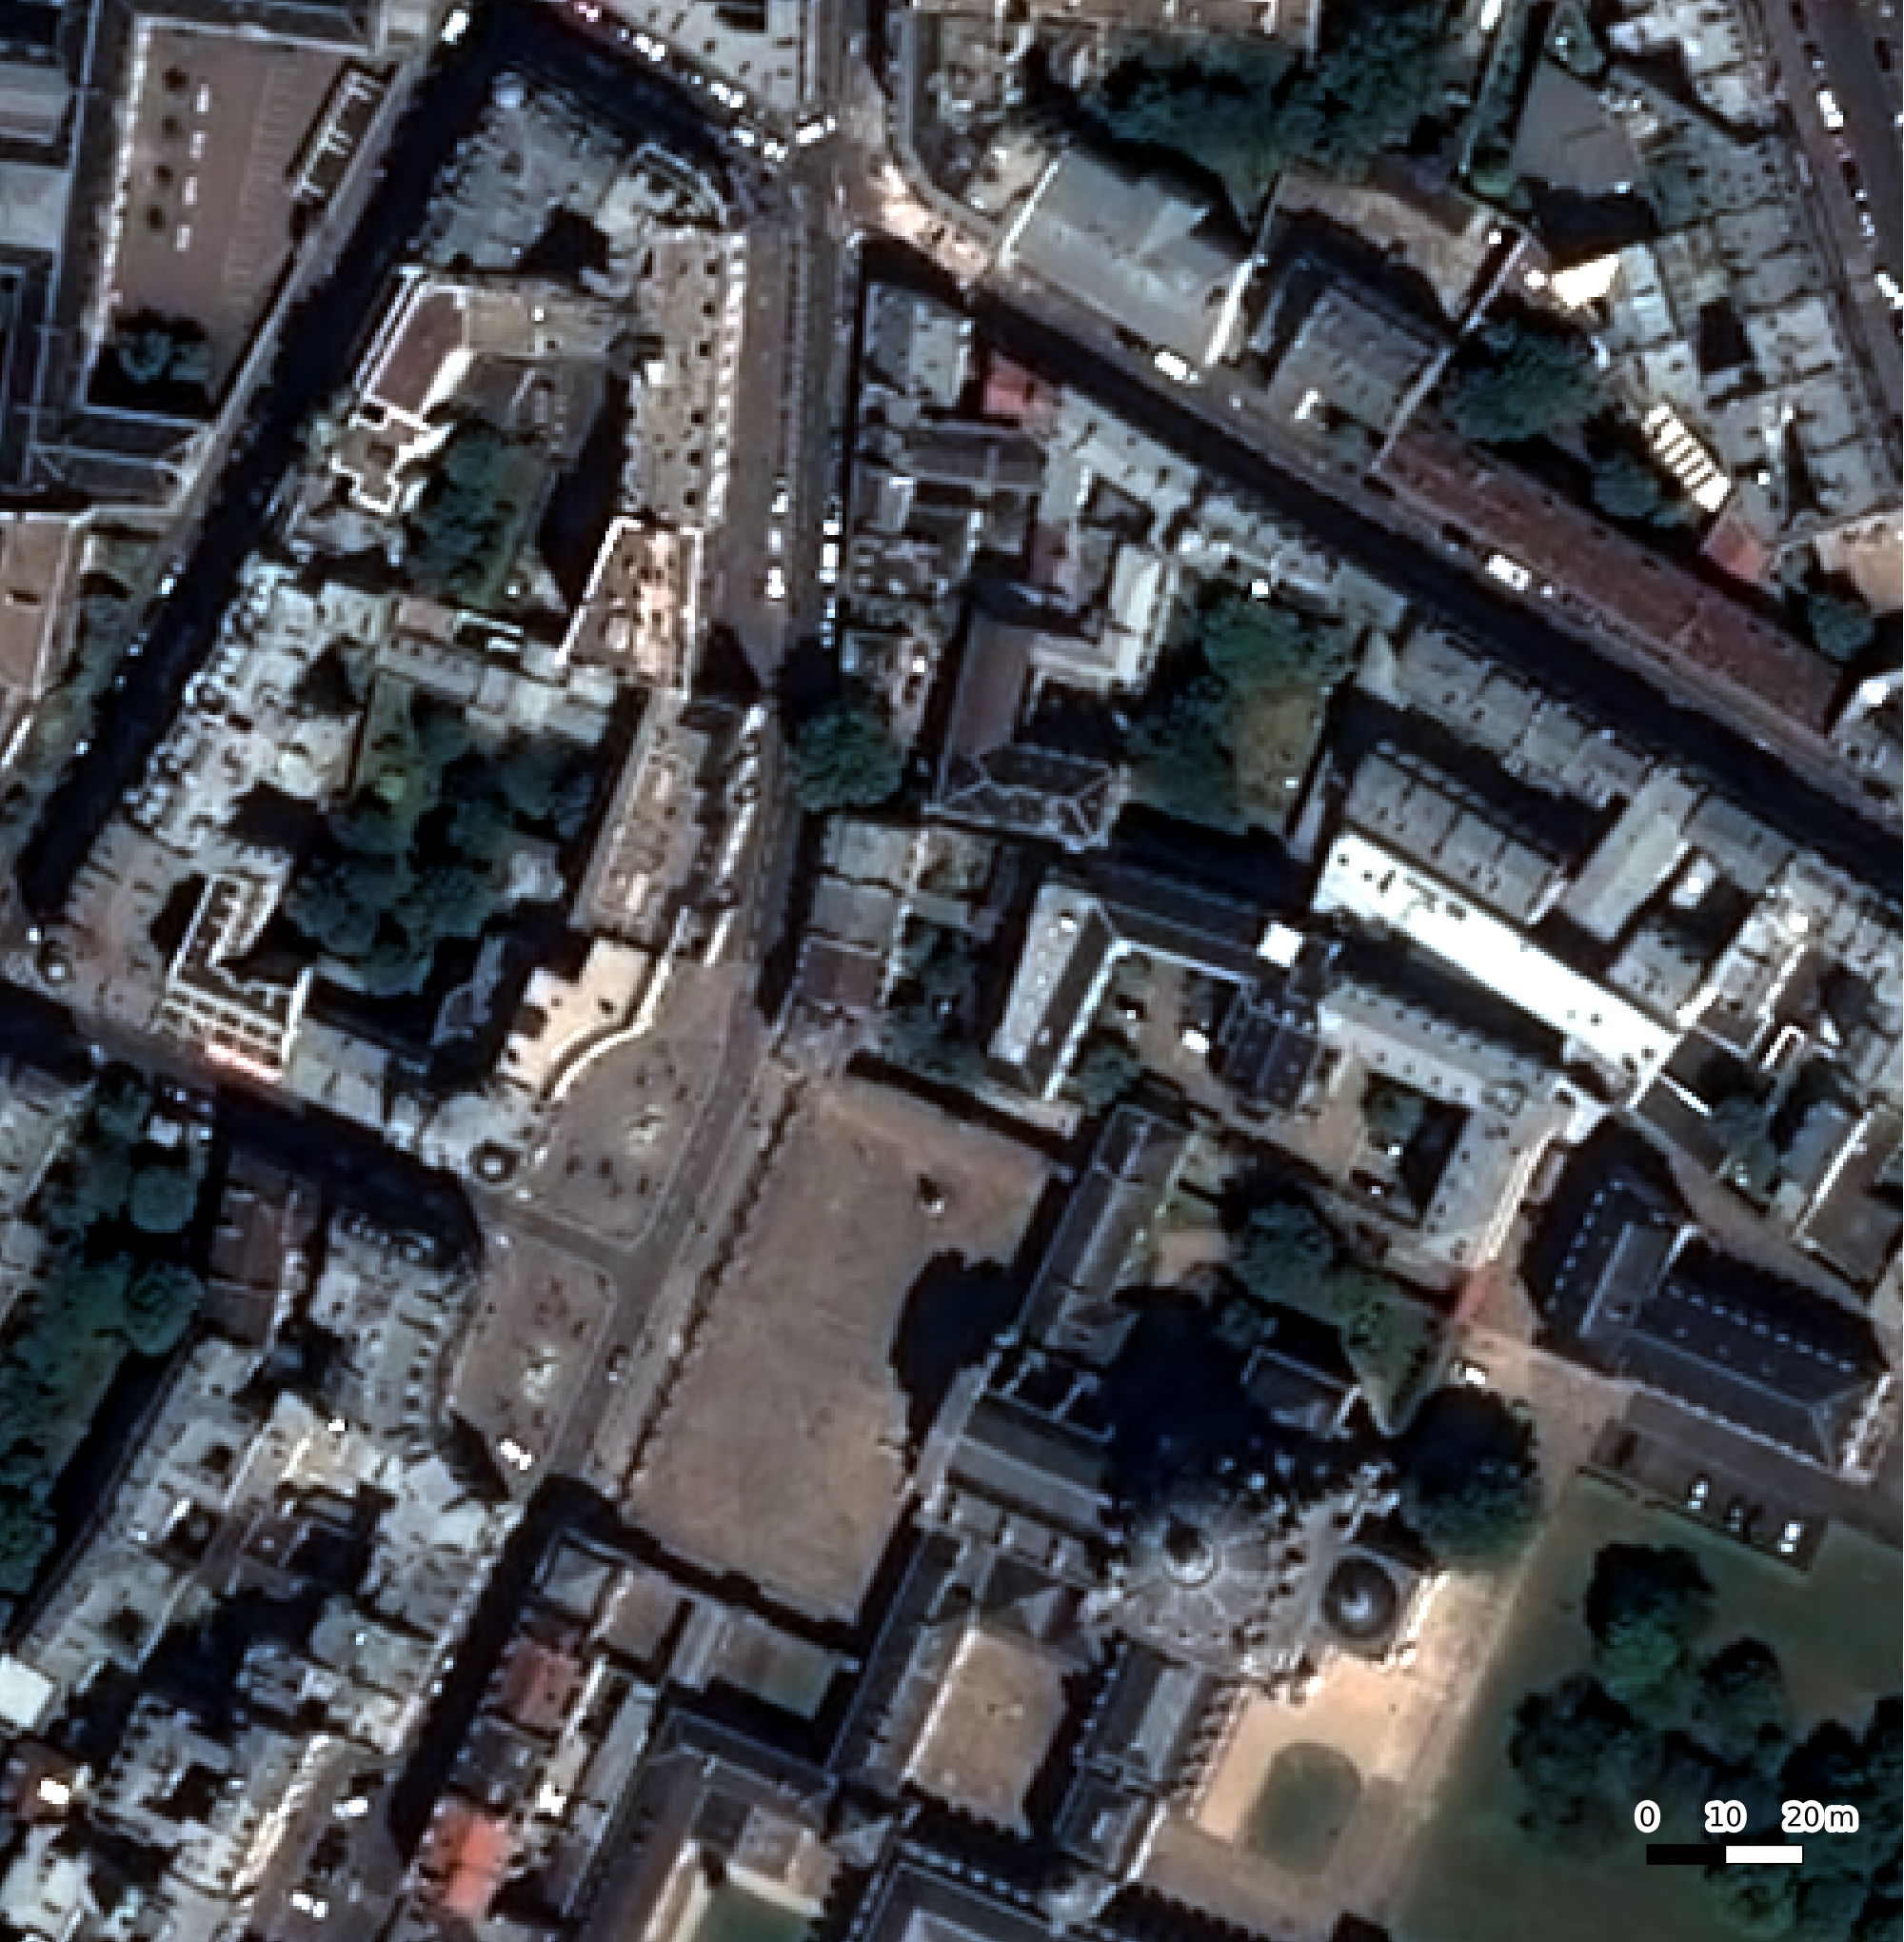
\includegraphics[height=6cm]{Images/0_Intro/Paris_Ortho.png}
        \caption{Pléiades image \copyright CNES 2017, Distribution AIRBUS DS}
        \label{fig:VDG_ortho}
    \end{subfigure}\hfill
    \begin{subfigure}[t]{0.5\linewidth}
        \centering
        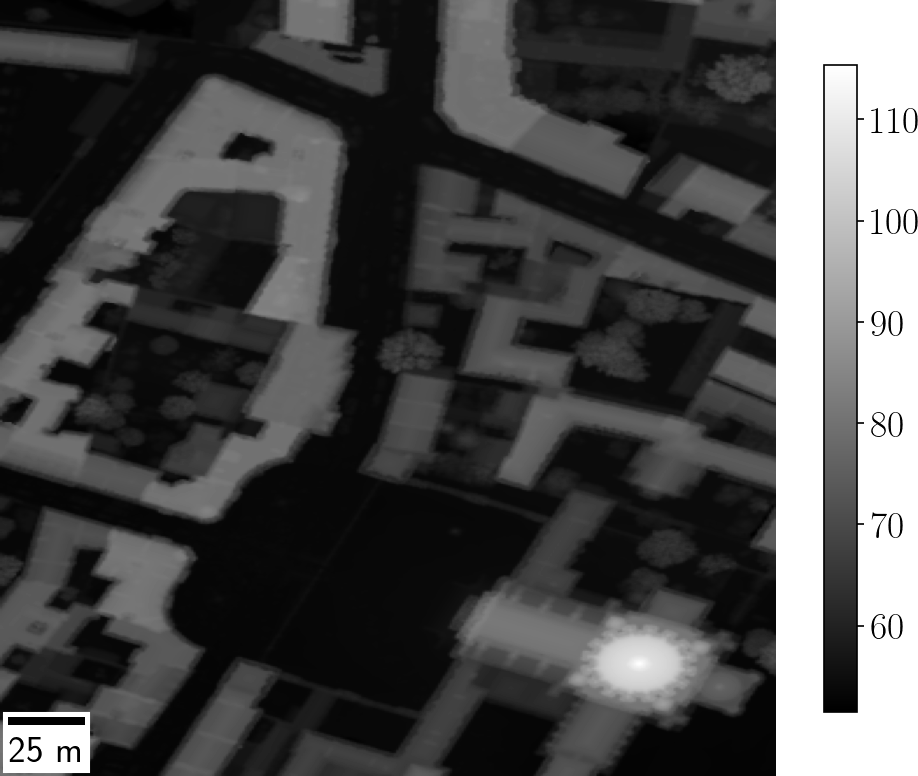
\includegraphics[height=6cm]{Images/0_Intro/Paris_DSM.png}
        \caption{Digital Surface Model from LiDAR HD}
        \label{fig:VDG_dsm}
    \end{subfigure}
    \caption{Satellite image over Val-de-Grâce, Paris at $0.5$m of resolution, and a DSM over the same area.}
    \label{fig:intro_dsm_example}
\end{figure}

There are multiple ways of creating a DSM. The first way is to use radar interferometry, as done by Sentinel-1 satellites \cite{geudtner_sentinel-1_2014} or the Shuttle Radar Topography Mission (SRTM) \cite{farr_shuttle_2007}. This method presents the advantage of being able to acquire data by day and night, even in the presence of clouds. Typical resolutions obtained are in the range of a few meters. For instances, the worldwide DSM produced by the SRTM mission has a resolution of $30m$. An other method for producing DSM are using LiDAR (laser sensors) \cite{khosravipour_generating_2016}. Using those sensors allows to obtain very good accuracy. For instance, the french institude IGN (\textit{Institut national de l'information Géographique et forestière}) is using LiDAR to cover the french territory with a resolution of $10$ points per $m^2$. However acquisitions campaigns such as this one are carried out using airborne vehicles, and are thus costly and take a lot of time. Finally, it is possible to construct DSM by means of (stereo) photogrammetry \cite{tao_comprehensive_2001}, \ie the science of recovering 3D information from optical images. For this method, images of a scene are acquired from different points of view, and depth information is recovered from the parallax effect between images. As current optical satellites have a sub-meter resolution, it is possible to massively produce DSM covering the globe using photogrammetry for a relatively low cost. Throughout this thesis, we will mainly consider photogrammetry as our mean to produce DSM.

In this context, CNES - the French Space Agency - is planning to launch 4 low-cost optical satellites with Airbus Defense and Space, in order to massively produce DSM using stereo photogrammetry. This mission, named CO3D (for \textit{Constellation Optique 3D}, \cite{melet_co3d_2020}), was conceived jointly with IGN to provide high resolution DSM over the globe, at a $50cm$ resolution.

CNES also developed a pipeline dedicated to process all images provided by the CO3D satellites automatically and at a very large scale. This pipeline is called CARS (``Chaine Automatique de Restitution par Stéréoscopie''), and is composed of many different image processing algorithms. As stated previously, the depth information is retrieved from the parallax effect between images, \ie the different movement of objects in-between images depending on their distance to the sensors. The quantification of this movement is done during a step called dense-matching, where we try to find the different positions of each pixel in multiple images. Dense-matching is therefore the core part of the CARS pipeline, and it is also a popular problem in computer vision in general (for autonomous cars for instance \cite{geiger_are_2012}).

Alongside DSM, on of the requirements of the CO3D mission is to produce a performance map indicating the estimated quality of each cell of the DSM. This motivated CNES to lead research which investigated the uncertainty amongst the CARS pipeline. The main objective of this thesis was to therefore to characterize and propagate the uncertainty throughout this photogrammetry pipeline. However, it was clear from the beginning that characterizing the uncertainty of every step of the pipeline was too much work one thesis, as many complex algorithms interact inside CARS. We thus mainly focused in the dense-matching step: being the crucial and hardest part of the pipeline, it is also the step that is the most determining for the final uncertainty.

\commanue{Bonne intro sur l'incertitude, bravo ! Il te faudrait une petite phrase ou deux de transitions sur pourquoi tu abordes maintenant l'incertitude}
As we will deal with uncertainty throughout this thesis, we first need to specify what we mean by uncertainty. Uncertainty is a situation where a measure or value of interest is not known, or not known with precision. It is subject to change, as additional information, measures or a different acquisition protocol may reduce how uncertain a value is. It can also be subjective. For instance someone maybe uncertain about the launch date of CO3D satellites while someone else working at the launch pad might have the answer. This highlights the fact that while everyone has an understanding of what uncertainty is, it encompasses very different concepts in nature. It is common to differentiate the various types of uncertainty by dividing it into two categories: stochastic (or random) uncertainty and epistemic uncertainty.

Stochastic uncertainty refers to every situation of purely aleatoric nature. For instance, the result of a coin throw, random noise on a CCD captor or the Brownian movement of a particle. An operator typically encounters this kind of uncertainty in a situation where they have access to many measures or observations of the same value of interest. It is usually modeled mathematically with a frequentist approach, using probability measures such as the uniform distribution, Gaussian distribution, Student's $t$ distribution \etc 

On the other hand, epistemic uncertainty refers to a situation where the value of interest is not known or ill-known due to a lack of knowledge. Think of the previous example with the launch date of satellites, or if someone was asked to guess Io's mass, one of the moons of Jupiter. There is no random process at stake here, and there is usually no point of acquiring multiple samples of the measure. Once the value of interest is known, the uncertainty usually no longer exists. It has been proposed to model this kind of uncertainty using a Bayesian approach for probability, by opposition with the frequentist approach. Probabilities here represent a state of knowledge, or degree of belief, one has over the value of interest. It can be updated with additional knowledge, thus leading to the notion of prior and posterior probabilities. We will see during this thesis that other model can be used to characterize this uncertainty, for instance \textit{imprecise probabilities} and more specifically \textit{possibility distributions}. It is note the first time that those models are considered for processing satellite imagery, as another thesis estimated land changes uncertainty using possibility distributions \cite{lesniewska-choquet_specialite_2020}.

Although uncertainty can be complex and expensive to compute, characterizing and quantifying it has many benefits. It provides additional information for better decision making and risk management. It can also allow for a better understanding of the underlying processes at stake regarding the value of interest. In many cases, uncertainty estimation is treated as a secondary objective in applications. However, jointly estimating a value and its uncertainty can lead to new strategies to reduce the uncertainty or sometimes even improve the performances of the main applications \cite{chen_learning_2023,jiang_unsupervised_2024}.

During this thesis, we both contributed to the field of photogrammetry and to the field of imprecise probabilities. Here is a quick overview of the contents that can be found in the following chapters:
\begin{itemize}
    \item Chapter \ref{chap:stereophotogrammetry} introduces the different stereo photogrammetry concepts considered in this thesis. It focuses on the stereo pipeline developed by CNES and its sources of uncertainty, which will be considered in our applications.
    \item Chapter \ref{chap:representation_of_uncertainty} will introduce the different uncertainty models considered in this thesis, mainly possibility distributions and copulas. The end of chapter \ref{chap:representation_of_uncertainty} and the following chapters constitute the main contributions of this thesis.
    \item In chapter \ref{chap:joining_credal_sets}, we propose different methods for creating specific multivariate uncertainty models based on the models introduced in chapter \ref{chap:representation_of_uncertainty}. We also study the relationships between the methods we introduced.
    \item Chapter \ref{chap:propagating} uses the concepts of chapter \ref{chap:representation_of_uncertainty} and the results of chapter \ref{chap:joining_credal_sets} to propagate uncertainties modeled by possibility distributions in a part of the dense-matching step of the stereo pipeline.
    \item Chapter \ref{chap:epistemic_uncertainty} also uses possibility distributions, but this time to characterize the uncertainty of the dense-matching step itself. Using this method, we are able to obtain confidence intervals at the end of the dense-matching step. Those intervals are then propagated to the end of the pipeline, to generate confidence intervals on the final DSM.
\end{itemize}

Allow us to make a small disclaimer: because our contributions concern two distinct fields of research, readers with a level of expertise in one field might be less interested in the second field. We tried, as much as possible, to write each chapter so it can be read and followed by everyone, although some details might need additional knowledge in a field of expertise. To help readers to navigate through chapters according to their center of interests, here is an attempt to classify each chapter into its field of research.
\begin{itemize}
    \item Chapter \ref{chap:stereophotogrammetry} focuses on stereo photogrammetry.
    \item Chapters \ref{chap:representation_of_uncertainty} and \ref{chap:joining_credal_sets} focuses on the modelling of uncertainty.
    \item Chapter \ref{chap:propagating} joins both fields, but leans a bit more towards uncertainty propagation than towards photogrammetry. 
    \item Chapter \ref{chap:epistemic_uncertainty} also attempts to join both fields of research, but focuses almost completely on photogrammetry.
    \item Chapter \ref{chap:results} presents the results of chapter \ref{chap:epistemic_uncertainty}, but does not belong in one field or another.
\end{itemize}

The rest of this section lists the contributions and research events that occurred during this thesis.

\noindent National conferences:
\begin{itemize}
    \item LFA 2022: ``Copules, probabilités inférieures et ensembles aléatoires : comment et quand les appliquer ?''  \cite{malinowski_copules_2022}
\end{itemize}
International conferences:
\begin{itemize}
    \item SMPS 2022: ``Copulas, Lower Probabilities and Random Sets: How and When to Apply Them?'' - \cite{malinowski_copulas_2022}
    \item ISIPTA 2023 (Special jury recognition Award): ``Uncertainty Propagation using Copulas in a 3D Stereo Matching Pipeline'' -  \cite{malinowski_uncertainty_2023}
    \item IGARSS 2024: ``Robust Confidence Intervals For Digital Surface Models Using Satellite Photogrammetry'' -  \cite{malinowski_robust_2024}
\end{itemize}
International journals:
\begin{itemize}
    \item International Journal of Approximate Reasoning: ``Uncertainty propagation in stereo matching using copulas'' -  \cite{malinowski_uncertainty_2024}
\end{itemize}
Not yet published pre-print:
\begin{itemize}
    \item : Available on ArXiv: ``Robust Confidence Intervals in Stereo Matching using Possibility Theory'' - \cite{malinowski_robust_2024-1}
\end{itemize}
Workshops, poster sessions \etc:
\begin{itemize}
    \item Belief 2022 conference: Poster presentation
    \item Workshop Imagin ``journée imprécision et incertitude en analyse et traitement d'images'': oral presentation
    \item SFPT ``Pléiades Neo: de nouveaux satellites pour de nouveaux usages'': oral presentation
    \item GdR IASIS ``Télédétection et Climat'': oral presentation
\end{itemize}

\pagebreak